I will define \acrfull{vr} and show the main characteristics of it through this chapter. Followed by listing a number of related projects that has been made in different places to immerse and show the user locations in different times. The last section will represent example projects that has been done in \acrshort{vr} in different places in the world focused on immigration, refugees and time traveling.   

\section{Virtual Reality}
Ivan Sutherland created a Head-Mounted Display in 1968 which displayed left and right views of a computer-generated 3D scene to the user, so that the digital scene remained static when the user's head was shifted. The images, as they were simple line drawings, were far from life. But as they were stereoscopic, the user had the impression of looking at a solid 3D object, which was the birth of Virtual Reality. In 1965 he published a paper entitled "the ultimate display" describing how computers would one day open a window to the virtual world for the user. \citep{Vince2011}.  

Virtual reality is a technology that is often regarded as a natural extension of 3D computer graphics with specialized input and output tools \citep{Jayaram1997}. Ryan (2001) defined it as an “interactive, immersive experience generated by a computer” \citep{Ryan2001}. And according to G.C. Burdea and Coiffet (2017) “it is a generated computer graphics used to create a realistic-looking world that responds to the user’s input (gestures, verbal commands, etc.)” \cite[p.20]{burdea2017virtual}. Instead of seeing a screen in front of them, the users will be engulfed in a 3D environment by virtual reality.“The scientific community has been working in the field of virtual reality (VR) for decades, having recognized it as a very powerful human-computer interface”\cite[p.19]{burdea2017virtual}. 

As shown in Figure \ref{fig:3I} In order to build a situation of virtual reality, three elements are needed:  immersion, interaction, and imagination. They are called the “3I’s” of virtual reality \citep{Hu2016,burdea2017virtual,Bamodu2013VirtualComponents}.

\begin{wrapfigure}{r}{0.30\textwidth} %this figure will be at the right
    \centering
    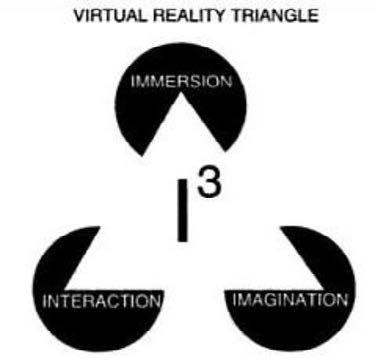
\includegraphics[width=0.28\textwidth]{3I}
    \caption{The 3I's of Virtual Reality - © 2003 by John Wiley \& Sons Inc. All rights
reserved}
    \label{fig:3I}
\end{wrapfigure}



1. \textbf{Immersion:} It is the situation of virtual reality in which the user feels inside the scene personally and immerses himself in the simulated virtual world.



2. \textbf{Interaction:} The user-to-virtual environment interactive feedback. Since it is an interface between man and machine, the system should immediately respond to the actions of the user.




3. \textbf{Imagination:} For a better user simulated experience, the scene structure and the construction of the environment were formulated with imagination.

\section{Types of Virtual reality systems} \acrshort{vr} technologies has been categorised into three main categories, Non-immersive system, semi-immersive system, and Immersive system, according to \cite{Bamodu2013VirtualComponents}. This is based on the system's level of immersion, interface, and components used.  

\textbf{Non-Immersive VR system}
It is also called the World system's desktop \acrshort{vr} system, Fishtank or Window is the least immersive and least expensive of the \acrshort{vr} systems because it needs the least complex components. This uses traditional graphics workstations with a screen, a keyboard, and a mouse, with modeling and \acrfull{cad} systems in its software areas.  

\textbf{Semi-Immersive VR system}
Use a relatively high-performance graphics computing system coupled with a large surface to display the visual scene, provide high immersion levels while maintaining desktop \acrshort{vr} simplicity or using some physical model. One such program is the \acrfull{cave} and the driving simulator is an application. 

\textbf{Immersive VR system}
 The immersive \acrshort{vr} system is the most expensive and provides the highest level of immersion, its components include HMD, tracking devices, data gloves, and others that include the user with computer-generated 3D animation that gives the user a sense of being part of the virtual environment. One of its features is digital house walk-through \citep{Bamodu2013VirtualComponents, Baus2014MovingReview}.

\begin{figure}[ht]
    \centering
    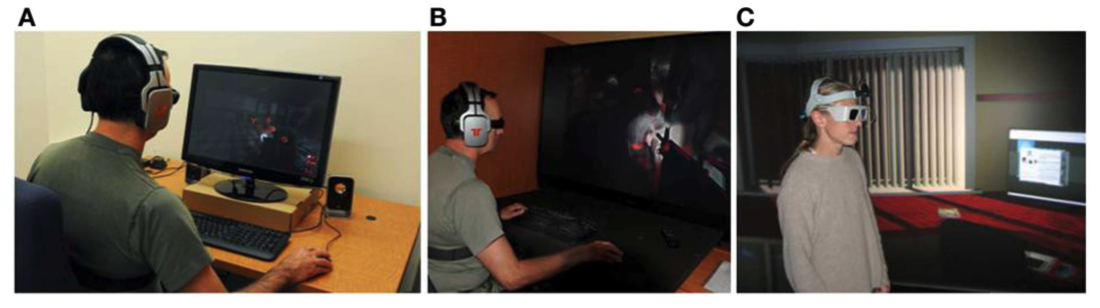
\includegraphics[width=0.98\textwidth]{images/vrsystem.png}
    \caption{VR Systems A: non-immersive system, B: semi-immersive system, C: Immersive system \citep{Baus2014MovingReview}}
    \label{fig:vrsys}
\end{figure}


\section{Presence in Virtual Reality} 
Due to powerful simulated influence, the user will experience emotional and physical response as if the virtual world happened physically, the sensation of being in a real place, as well as the perception of validity, getting the sense that the scenario is taking place. Although the user knows that the virtual world is just a simulation, these illusions occur. \acrshort{vr} has been one of the main trends in the evolution of presence \citep{Waterworth2014, Steinicke2016}.
Human-computer interaction ranges from purely visual interaction to differentiated contact that the user can communicate with objects in virtual reality with the perceptions and cognitive processing capacities experienced in the real world, and the sensation is similar to the changes in the natural world \citep{Hu2016}.
\acrshort{vr} gives the user the ability to control, move and look in the virtual world, which has a significant impact on the level of presence, hence the greater the user's sense of immersion \citep{William}. \say{When we feel strong mediated presence, we react emotionally and
bodily (at least to some extent) as if the virtual world existed physically}\cite[p.4]{Waterworth2014}.


We need to understand the \acrfull{fov} and the \acrfull{for} for a human to achieve a significant level of immersion for the user. The human \acrshort{fov} is about 200 degrees with a binocular overlap of 120 degrees. The field of view of the display is a measure of the angular width of the vision of a user that is covered at any time by the display as shown in Figure \ref{fig:field}. Due to the edge of the screen, the field of view is reduced in a three-sided \acrshort{vr} projection, but it is 100\% if the user looks forward to it. Nevertheless, throughout the three-sided stationary projection, the stereo range is broader, several \acrlong{hmd}'s provides a 100-120 degrees of \acrshort{fov} which is a sensible part of the human visual range. Even though the stereo overlap is very essential and can differ in \acrshort{hmd}'s where the two displays are more or less broadly separated, it will be difficult to perceive stereopsis if the overlap between the two eyes is as small as 30 degrees \citep{William}.
If the user moves towards an object, the ciliary muscles adjust the lens shape to handle the emitted light waves to keep a picture in focus. The eyes also intersect automatically to ensure that the refracted images fall on the two retinas similar areas. The cause of stereoscopic vision is this method of projecting an object to specific locations on the two retinas. The discrepancy between the retinal images is termed binocular disparity and is used to measure distance, resulting in a three-dimensional context \citep{Vince2011}.

\begin{figure}[ht]
    \centering
    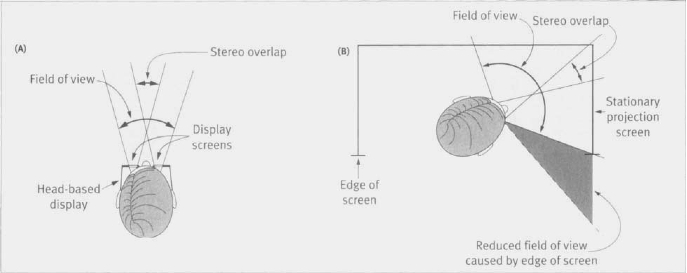
\includegraphics[width=0.90\textwidth]{Fod.png}
    \caption{Field of View - \citep{William}}
    \label{fig:field}
\end{figure}


\begin{figure}[ht]
    \centering
    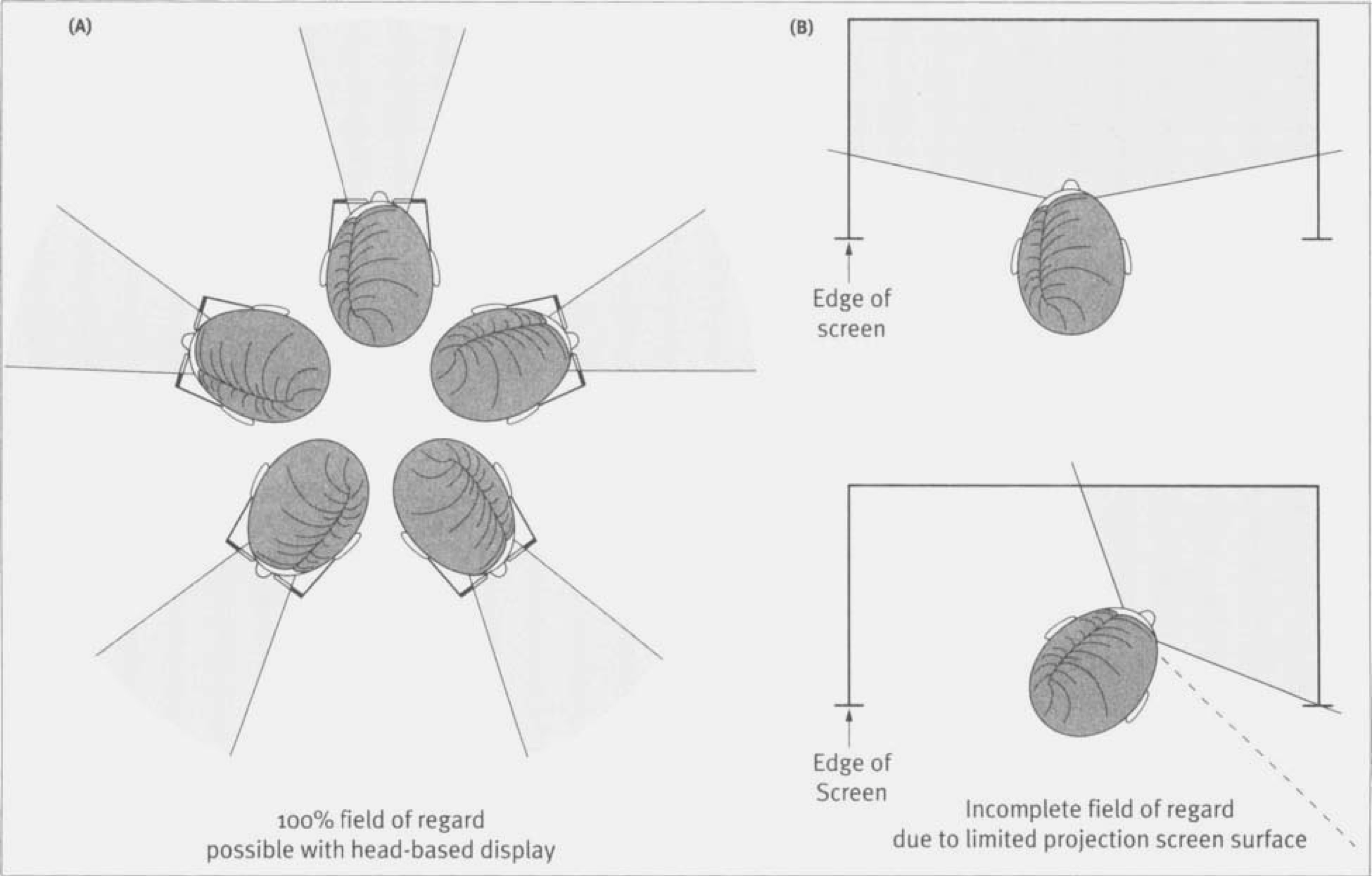
\includegraphics[width=0.90\textwidth]{fov.png}
    \caption{Field of Range - \citep{William}}
    \label{fig:fod}
\end{figure}

The \acrfull{for} is the amount of space within the virtual world that surrounds the user. As shown in Figure \ref{fig:fod}, due to the displays that always face the user's eyes, the \acrshort{for} in the \acrshort{hmd} is 100 percent, regardless of the direction that the user stares at, the virtual reality would always be in front of his eyes. In the three-sided \acrshort{vr} projection, the \acrshort{for} is usually less than 100 percent because the virtual environment will always need projectors and it will not be dynamic in motion as the \acrlong{hmd} \citep{William}.

An \acrshort{hmd} is nothing but a stereoscope, which uses not just pictures but animated video clips as well. What is significant, however, is that the images seen by both eyes must overlap and stereoscopic vision is experienced in this field of overlap \citep{Vince2011}.
This stereo-overlap zone is shown in Figure \ref{fig:field}. Since the two images are captured from two different visual locations, the brain uses these variations to create a single image containing information about distance \citep{Vince2011}. Thus, the use of \acrshort{hmd}'s could have its repercussions, e.g. a low latency monitoring "not more than 2ms (millisecond)" is needed to adjust the screen picture to the viewer's physical movement  also to prevent movement discomfort because high latencies have serious negative consequences on simulation, e.g. vomiting, nausea or vertigo \citep{burdea2017virtual, Vince2011, Steinicke2016}.

Smartphones have created a technological revolution, merging communication and computing devices, where they are small in scale and can fit into the pocket of the user.The high computing power permitted in smartphones is adequate to handle the \acrshort{vr} world, thereby allowing a lightweight and realistic \acrshort{vr} interface and web renaissance of \acrshort{vr}. The main elements of smartphones today, such as high-density display panels, gyroscopes, and accelerometers, are installed in most models and therefore cost only a fraction of the Virtual reality system value in the early 1990s \citep{Steinicke2016}. 



  
\section{Related Work}

Virtual reality is a technology that offers users with multiple benefits and displays successful results in various aspects. Virtual reality is also useful for simulating inherently dangerous activities (e.g. coal mining) or expensive equipment (e.g. aircraft) tasks. Without compromising their safety, users can perform hazardous tasks. With a risk-free environment, virtual reality allows users to make and take decisions \citep{Aguinas2004}. While it is a risk-free environment, such as surgical practice, it has enabled its experiences by researchers in education. Traditionally, medical education apprenticeship has been done under the guidance of a professional physician while the surgical trainee trains to perform surgery. Virtual reality learning reduced the time required to complete a mission, improved accuracy and reduced errors \citep{Ks2009}. Virtual reality captures the curiosity of the student. They find engaging and walking through a virtual environment exciting and challenging. Students are able to study in-depth and make new findings. This allows the disabled to engage in an atmosphere of exploration and training. We can do tests in chemistry and physics and practice how to do them \citep{Pantelidis2010}. Virtual rehabilitation described as treatment delivery using the hardware and simulations of Virtual Reality. It is helpful for people with post-traumatic stress disorder (PTSD) or patients who are afraid of flying or other fears. According to 
\cite{Burdea2003} 92 percent of people who were afraid to fly maintained their success and flew on flights \citep{Burdea2003}.

Virtual reality has a positive effects in social and psychological directions, for instance it can reduce anxiety for people who have the fear of public speaking. \cite{Chang2019StereotypeOutcomes} discussed how women achieved higher scores in math when they studied math over a virtual environment and they used a male avatars in \acrshort{vr}. Therefore, avatars can affect interpersonal dynamics by incarnating a minority race, therefore it would decrease the bias against the minorities \citep{Markowitz2018ImmersiveChange, Chang2019StereotypeOutcomes}.   

 VR presents us with the ability to go further than these physical limitations. Within VR, individuals can break laws of physics to alter their appearance, skills, and atmosphere. Immersive virtual reality technology makes it possible to "change the nature of social interaction". Users can distinguish their actual behavior and appearance from their simulated representations, contributing to behavioral and social implications for both the digital and physical world \citep{Shriram2017VirtualBehavior}.
Several projects will present the role of virtual reality in accomplishing new experiences and enhancements in some fields.

\textbf{The Machine to be Another} \footnote{The Machine to be Another - \url{www.beanotherlab.org}} : A system of virtual reality that enables people to experience the world through the eyes and body of another person. Cognitive science, performance, and virtual reality make it possible for users to see themselves in a different body while interacting with the surrounding space and receiving realistic feedback. Based on long-term studies on how compassion can be encouraged in resolving issues such as cultural bias, diversity, conflict resolution, and body extension among others. The system also functions as a consequence of narrative, also a very useful framework in psychology and health care.
The system is designed for an open community of creators, scientists, and individuals with a common dream of building an empathic society. The BeAnotherLab's purpose is to encourage human integration through technical and scientific knowledge.

\textbf{Chernobyl VR} \footnote{Chernobyl VR - \url{www.chernobylvrproject.com}} : Chernobyl VR Project is made by The Farm 51,  it is integrating video game with an application for instructional and storytelling film. It is the very first virtual tour around the Chernobyl and Pripyat area. The project has been designed with state of the art technologies like 3D scans of locations and buildings, spherical photography, stereoscopic videos. 


\textbf{IrisVR} \footnote{IrisVR - \url{www.irisvr.com}} : A VR platform that enables engineers and customers to experience the designs in a space of real scale. IrisVR captures and transforms every 3D file into a walkable VR world. Iris is compatible with multiple Head-mounted displays, therefore the users can have meetings inside the space since Iris supports a multi-user experience provided with a reliable voice chat and a shared virtual environment for presentations and design reviews.


\textbf{AVR EON reality} \footnote{Eon Reality - \url{www.eonreality.com}} : EON Reality created eight AVR training modules for NTU students and staff in the chemistry laboratory. Using a head-mounted display in virtual reality, students and staff can improve their awareness and manage different disaster situations remotely without any of the potential hazards or costs.EON Reality's Virtual Trainer solution provided risk-free safety and prevention training for some of the most common chemical laboratory emergencies, from preventing and controlling chemical hazards to protecting the health and safety of colleagues within the laboratory.




\section{Example projects}

\begin{wrapfigure}{r}{0.30\textwidth}
    \centering
    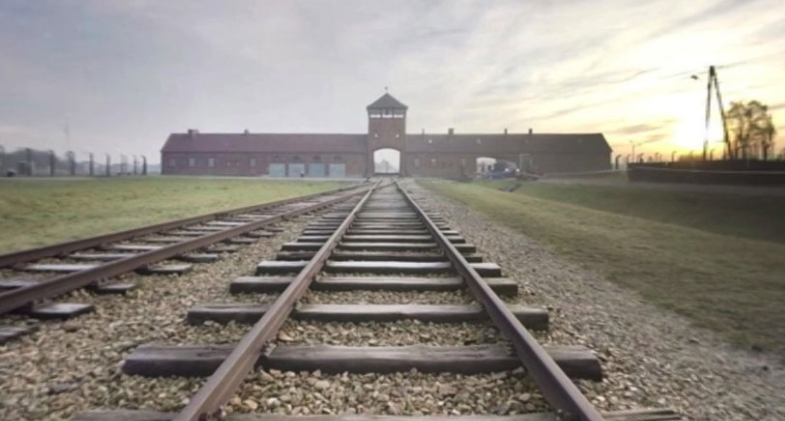
\includegraphics[width=0.30\textwidth]{images/Auschwitz2.png}
    \caption{Auschwitz concentration camp - © wdr.de}
    \label{fig:awsch}
\end{wrapfigure}
\textbf{Auschwitz Virtual Tour}\footnote{Auschwitz VR Tour - \url{www.youtube.com/watch?v=EOM_CxAKB_Y}}: The German broadcasting institution WDR made a 360$^{\circ}$ documentary in Auschwitz concentration camp. Within the documentary, some Holocaust survivors tell their stories. While listening to the stories and seeing the different locations in the camp the user could feel the fear and horror that people suffered from. The video immerses the user through the sound of the surrounding environment in the camp, you can hear the wind and the sound gives a slight feeling of the cold weather over there. The experience is immersive, but there is no interactivity with the user.

\begin{wrapfigure}{l}{0.30\textwidth}
    \centering
    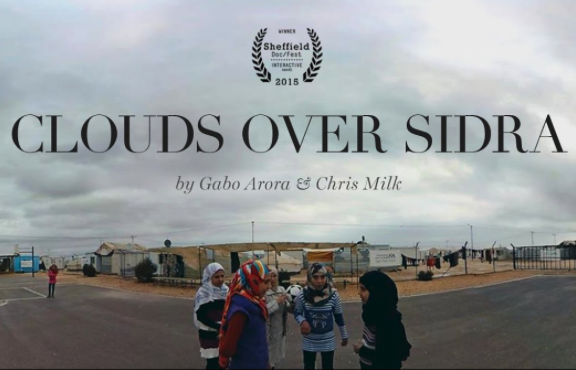
\includegraphics[width=0.30\textwidth]{images/clouds.png}
    \caption{Clouds over Sidra - © 360filmmaking.com}
    \label{fig:sidra}
\end{wrapfigure}

\textbf{Clouds over Sidra}\footnote{The Za’atari camp VR Tour - \url{www.youtube.com/watch?v=mUosdCQsMkM}}: A 12 years old girls’ daily life story at the Za’atari refugee camp in Jordan
showed in virtual reality. The camp is a home for 80,000 Syrian refugees, half of them are
children(“Syrian Refugee Crisis – UN Virtual Reality,” 2015). The documentary was made by
the United Nation to raise awareness about the Syrian crisis. The video contained a number
of short videos from different parts of the camp, and it’s being synchronized while Sidra
narrates her story.
It is more like watching a video with empathy than being immersed, but
the video presents the real life of the camp. Although the difference that while watching and
listening to the story, the user observes the people how they actually survive and live in the
camp. Therefore, the user does not have to imagine how is life over there.



\textbf{Carne y arena}\footnote{Carne y Arena Trailer - \url{www.youtube.com/watch?v=zF-focK30WE}} : A highly professional
Virtual reality project that puts viewers
into the harsh life of an immigrant. The
user is placed among a group of
Mexican immigrants passing the
borders into the U.S. It was written and
directed by Alejandro G. Iñárritu. It Is a
full virtual reality experience; the user
needs to reserve an individual session
on the website. According to Pinotti (2017) you go in a dark room; your feet are on the sand (coarse grain, rough feeling) then, two assistants welcome you and provide you with the
necessary devices: an Oculus Rift headset, a backpack connected via cables to a powerful
computer and you are ready to be caught up in a nightmare \citep{Pinotti2017}. The project is
subtitled by ‘Virtually present, Physically invisible’. 

\begin{wrapfigure}{r}{0.30\textwidth}
    \centering
    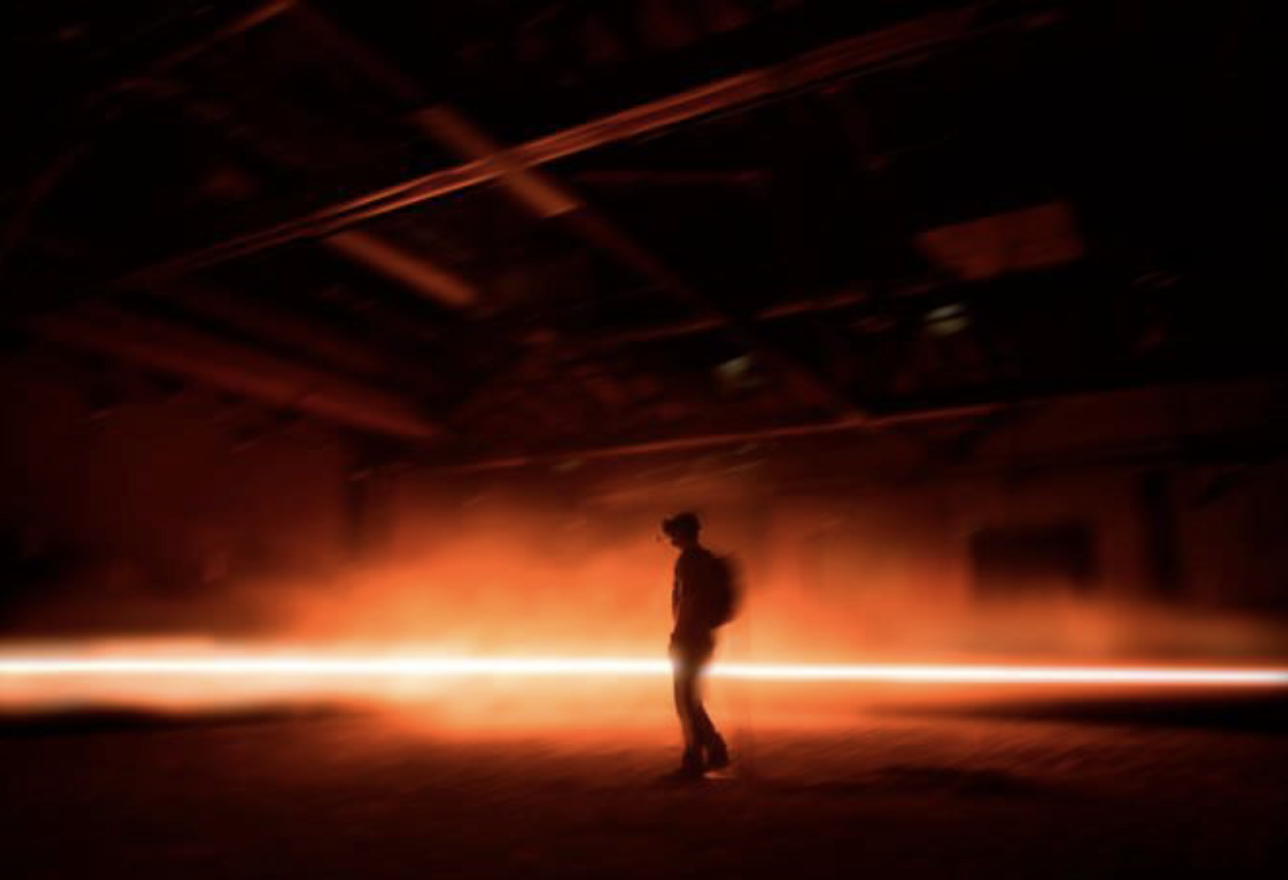
\includegraphics[width=0.30\textwidth]{images/carne.png}
    \caption{Carne y Arena—A user in the experience, 2017- © Emmanuel Lubezki}
    \label{fig:carne}
\end{wrapfigure}

Pinotti (2017) defined, Virtually present:
“you are transported in the middle of the desert, among men, women, and children who try
their voyage of hope”. Physically invisible: “you are present, but nobody sees you and after a
while, you start to feel the need to be noticed and seek acknowledgment of social
recognition” \citep{Pinotti2017}. The project was developed with high technology, like 3D
modeling, visual effects, sound. The interaction of the user and the feeling of “being there”
by placing the user in a special environment, leads to a unique experience of immersion.


\begin{wrapfigure}{r}{0.20\textwidth}
    \centering
    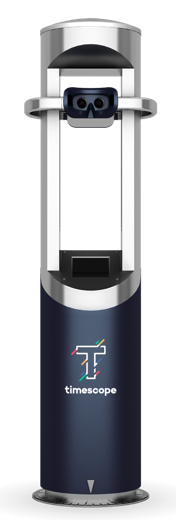
\includegraphics[width=0.16\textwidth]{timescope.png}
    \caption{Timescope terminal - © timescope.com }
    \label{fig:timescope}
\end{wrapfigure}
\textbf{Timescope}\footnote{Timescope - \url{www.timescope.com}} : A \acrshort{vr} terminal that installed in the street. It gives the user the ability explore the location in a different time. The terminal first installed at the Place de la Bastille in Paris. Where nothing remained of that historic place since it was demolished in 1789. Timescope developed this \acrshort{vr} terminal. Thus, it gives the people the ability to travel back in time and see the Bastille in 1416. Where it was first completed, or to 1789 where it was seized by revolutionaries. The 360 images and videos that are provided in the Timescope terminal gets the user immersed.

In different locations, the terminal also provides futuristic projects, to discover what would the location look like in the future \citep{Hiner2016HowTechRepublic}. 

\textbf{Palestine 360}\footnote{Palestine 360 - \url{www.360.ps}} : A platform that based on WebVR technology. It shows 360 images from different sites and locations in Palestine. The website gives the user the ability to use VR glasses to experience the 360 high quality images. The  images show not only historic locations but also restaurants and hotels. Some locations have background music and sometimes a narrator explaining the visited site. Some cities have a large-scale map on the right-side inside the VR experience. In a few scenes there is a location-pointer where the user can use the gaze feature as a click to get transported to a new scene. 


\textbf{Palestine VR App}\footnote{Palestine VR - \url{www.pipd.ps/2019/10/28/download-palestine-vr}} : The Application shows videos of real-life in Palestine. Each city in Palestine is represented by a different person. The presenters are holding the 360 camera while they walk around the city or the location. The app inculded videos from different cities Jerusalem, Hebron, Gaza City, Bethlehem, Ramallah and Khan Al Ahmar. Videos needs to get downloaded each time you use the application. thus, it might take some time to load the content on a slow internet connection. The Application has a different kind of a user interface when you activate the VR glasses mode. It has a gaze feature for selection, and the user can be transported between the scenes. Either by selecting the next scene by the bottom down video controllers or by getting back to the menu. 

\textbf{Time Ride}\footnote{Time Ride - \url{www.timeride.de}} : A guided tour that travels with the user in a different old times in different locations around Germany. Timeride is a physical location for public and tourists so they can see the city in a different scope of time. Timeride exist in Cologne, Dresden, Munich and Berlin. In Cologne the user will experience the imperial age of the city while siting in a tram cabin. While in Dresden the user will travel back to the Baroque era in 1719. The user will witness Bavarian history in Munich while sitting in a peacock wagon. Also in Berlin the user will enjoy a journey in the 80's.


\begin{figure}[ht]
    \centering
    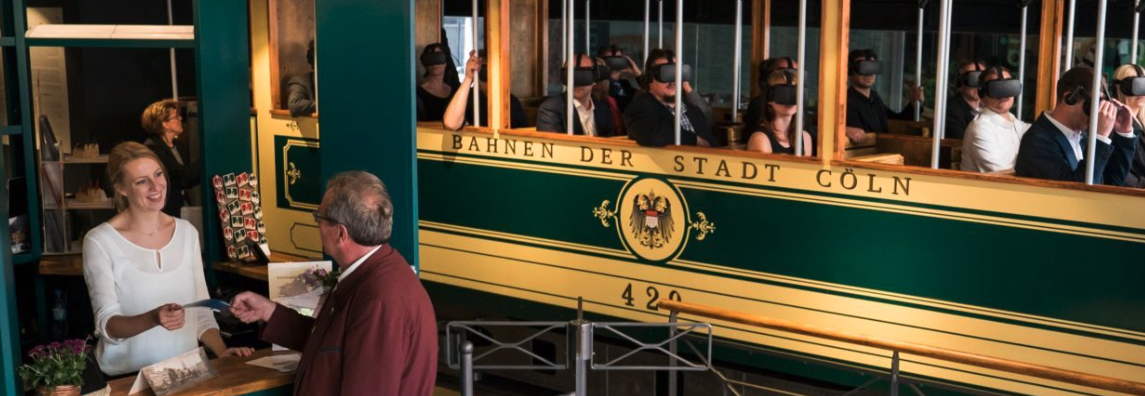
\includegraphics[width=0.98\textwidth]{images/timeride.png}
    \caption{Timeride in Cologne - © timeride.de }
    \label{fig:time}
\end{figure}
